\section{WC 30/6/25}

\subsection*{Overview:}
With my project having launched last week I am now waiting for a couple of weeks to see how users interact with the site and what feedback they provide. During this waiting period I am focusing on improving the presentation of my EPQ report documentation so that it is fluid to navigate and most importantly easy to understand.

I have worked hard throughout the EP period to keep my OneNote note store well-organised in numerous clearly-labelled Sections so that I can easily find the necessary information however I have found that whilst conducting a test export to PDF for final submission (as advised by my Mentor) the produced document felt untidy, thrown together and worst of all unorganized. I know that the presentation of the final report is not a marking criterion within the EPQ however, having spent so much time building and documenting a platform I am hugely proud of, I wanted to produce a report that I could be equally proud of showcasing to others.

\begin{figure}[H]
    \centering
    \begin{minipage}{0.3\textwidth}
        \centering
        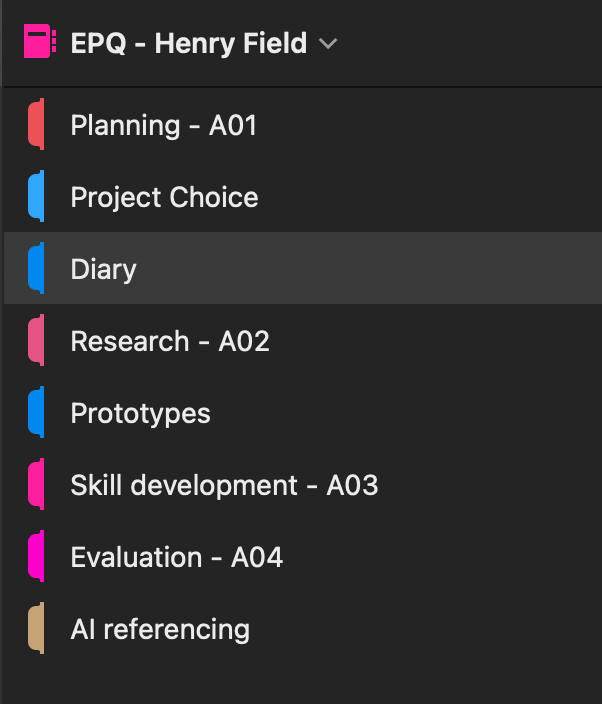
\includegraphics[width=\linewidth]{Diary/35_WC_30-6-25/media/OneNoteFolders.png}
        \caption{OneNote sections}
    \end{minipage}\hfill
    \begin{minipage}{0.48\textwidth}
        \centering
        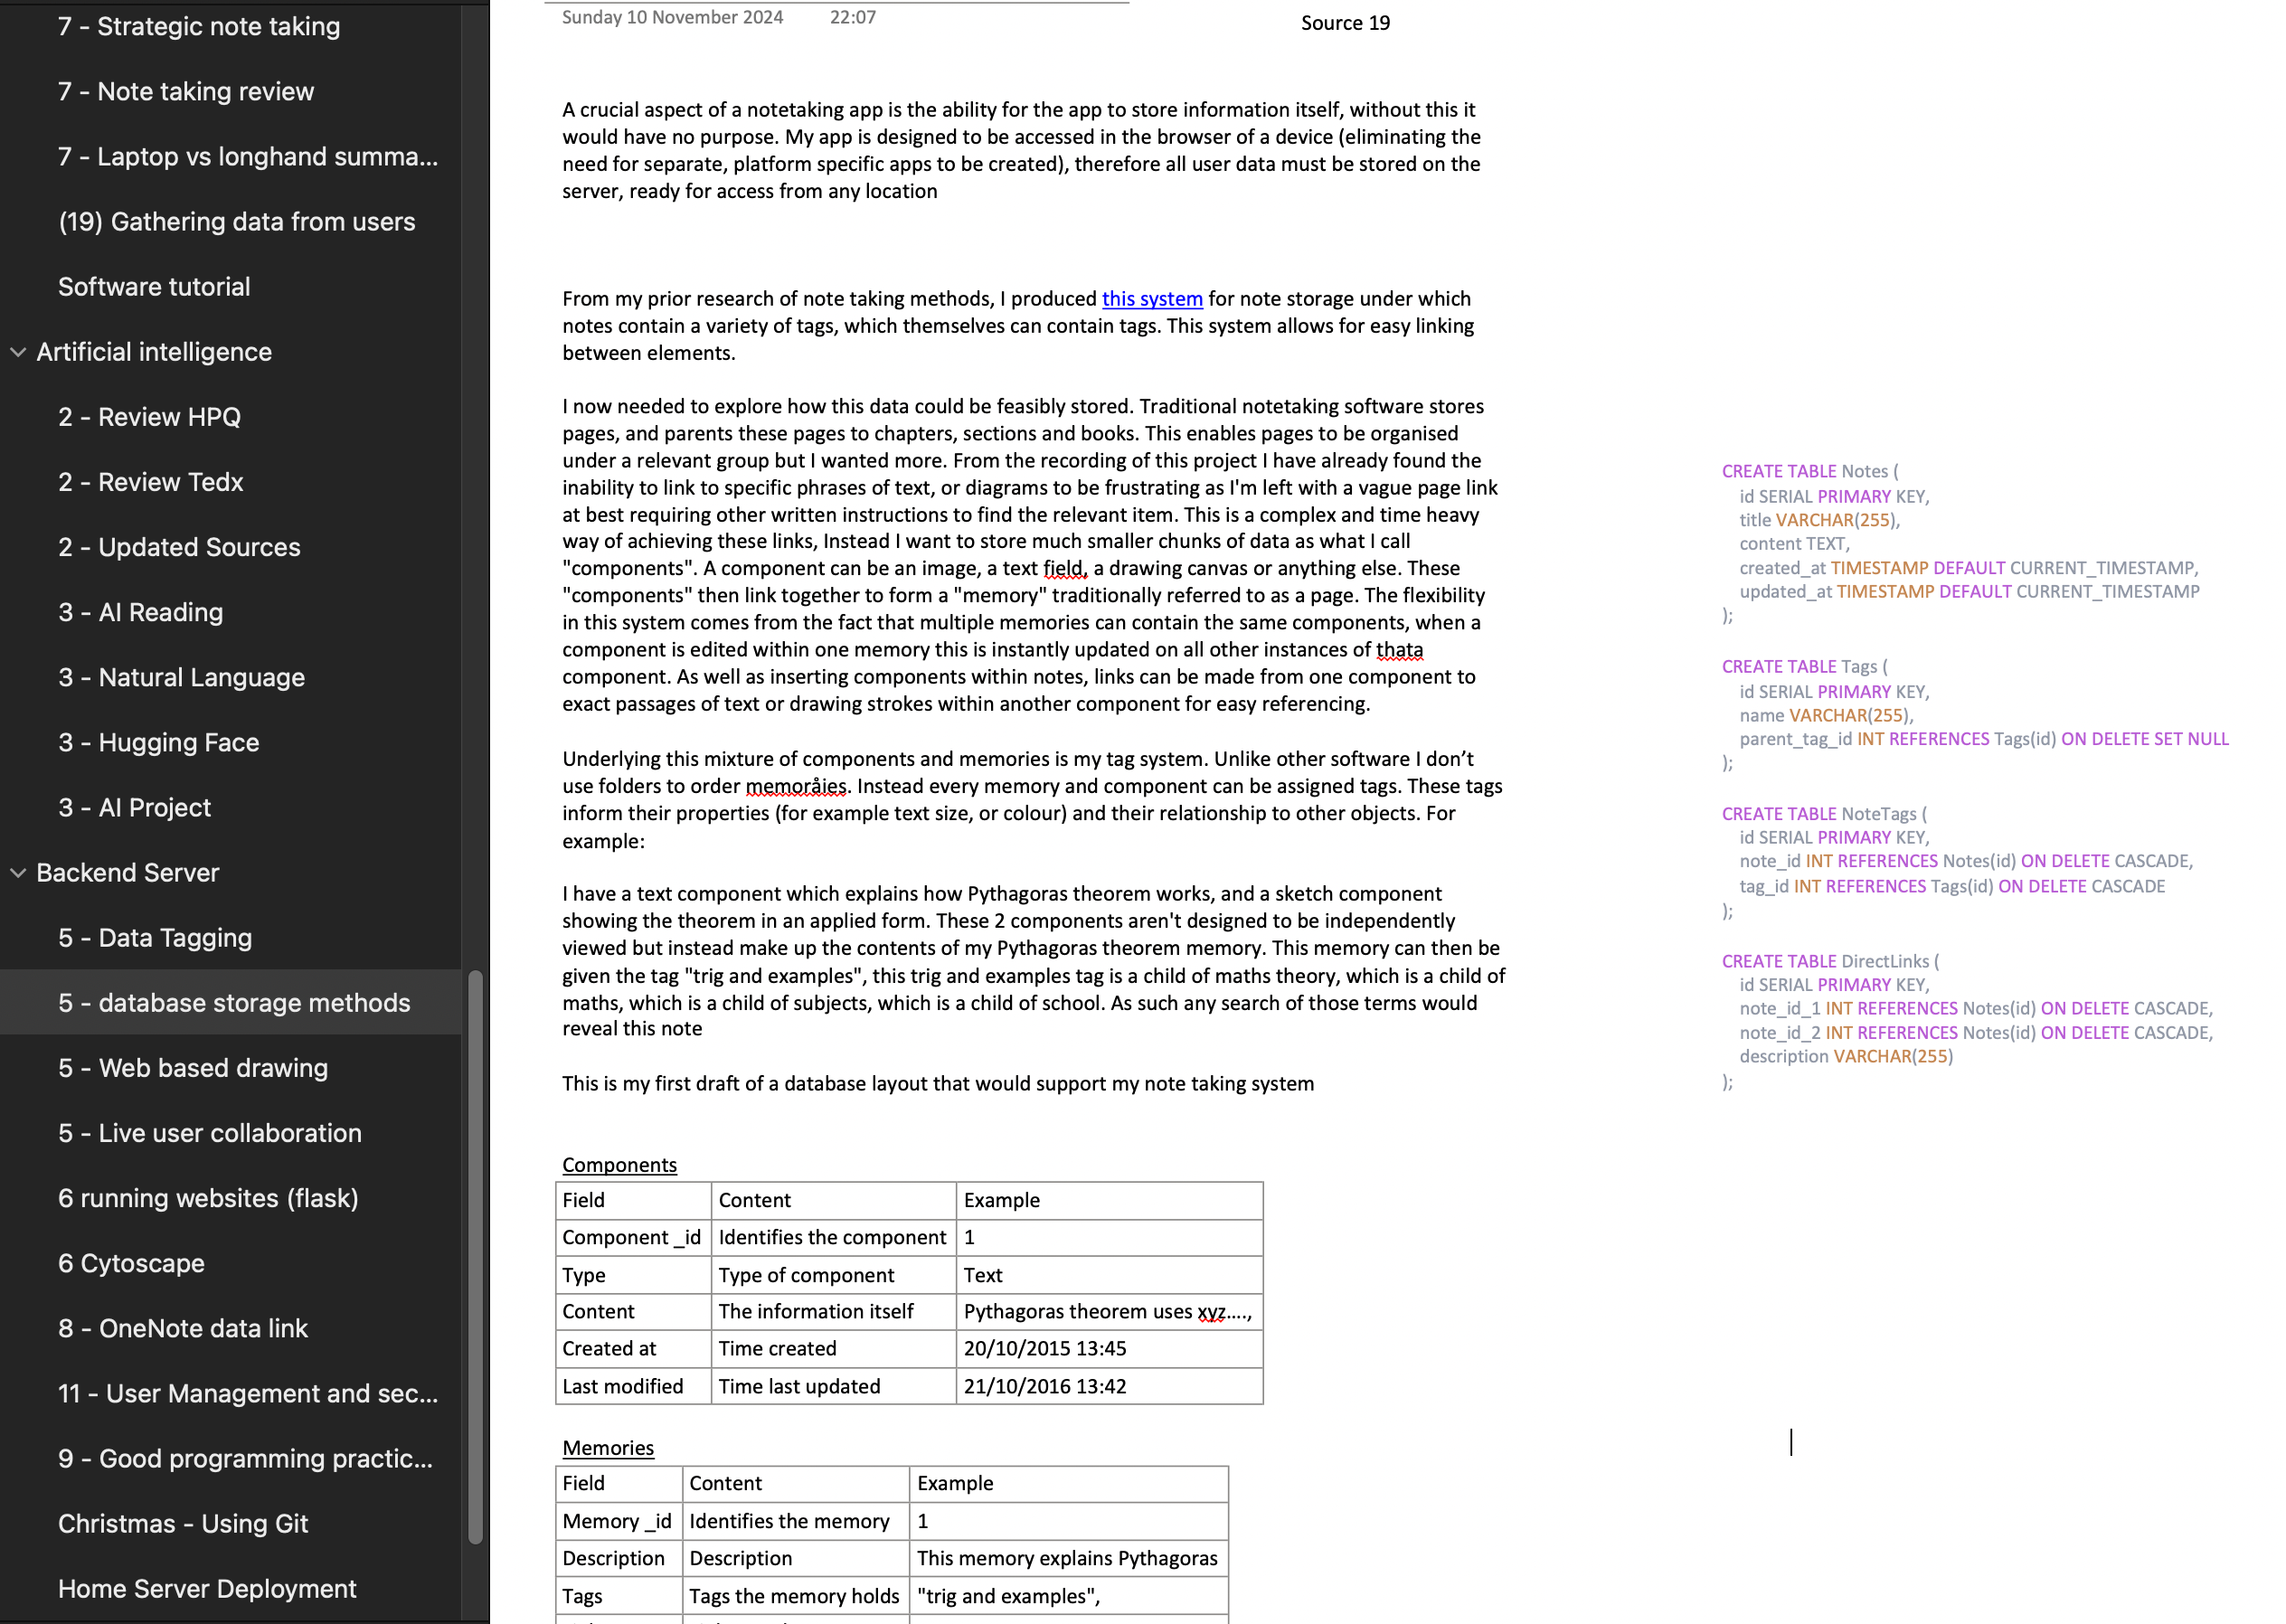
\includegraphics[width=\linewidth]{Diary/35_WC_30-6-25/media/folderOrg.png}
        \caption{Structure within folders}
    \end{minipage}
\end{figure}

Within various research pieces, for example, I had created sprawling tables, diagrams and handwritten notes that did not transfer cleanly into a A4 report and caused the entire OneNote page to 'zoom out' making it difficult to read and understand the information I processed. Equally, frustratingly I would be unable to create a thorough contents page (making it difficult to locate various elements within my report) and I would be unable to link to other pages within the report such as this: \nameref{sec:ProjectIdeas} - which is a hugely useful feature when presenting chronologically ordered information such as this diary in combination with various research pieces, prototypes and evaluations.

Hopeful to find a system that would allow me to present my report in a more professional manner I spoke with my parents to understand the process they had used to produce their own reports during their time in academia. I was very fortunate that my father could remember back "a fair few years" to a system called \LaTeX{} and \textit{spoiler} That is what I have switched to using to beautifully format this very document. During this conversation he did warn me that it was a fairly complex system to use however I quickly learnt that it was still the standard used by most universities / academics for reports and so learning this skill now would serve me well in later life. I have therefore added document formatting to my skills evaluation and began researching the fascinating world of \nameref{research:Latex}.

Whilst I didn't yet start migrating all of my content from OneNote to \LaTeX{} this week (which will likely be a fairly manual process) as I wanted to ensure I started in the most optimal way, I did decide upon my desired report structure which is as follows:

\begin{enumerate}
    \item PPR
    \item Project Commentary
    \item Project Choice
    \item Planning
    \item Diary
    \item Research
    \item Prototypes
    \item Skill development
    \item Evaluation
    \item Video Presentation
    \item Bibliography
\end{enumerate}

I hope this new structure makes it easier to navigate my report and find the information examiners are looking for. I have also started to create a new \LaTeX{} file for each section so that I can easily add content as I go along.

I have also made a quick draft title page for my report which I am very pleased with. Whilst my Art skills are very poor I found this lovely illustration called Washing the Feet (from the Dusty World) online here: \cite{WashingFeetDusty} and I have used it as the basis for my title page. I used my prexisting photoshop skills to extend the image upwards and add some birds which nicely frame my report title.

\begin{figure}[H]
    \centering
    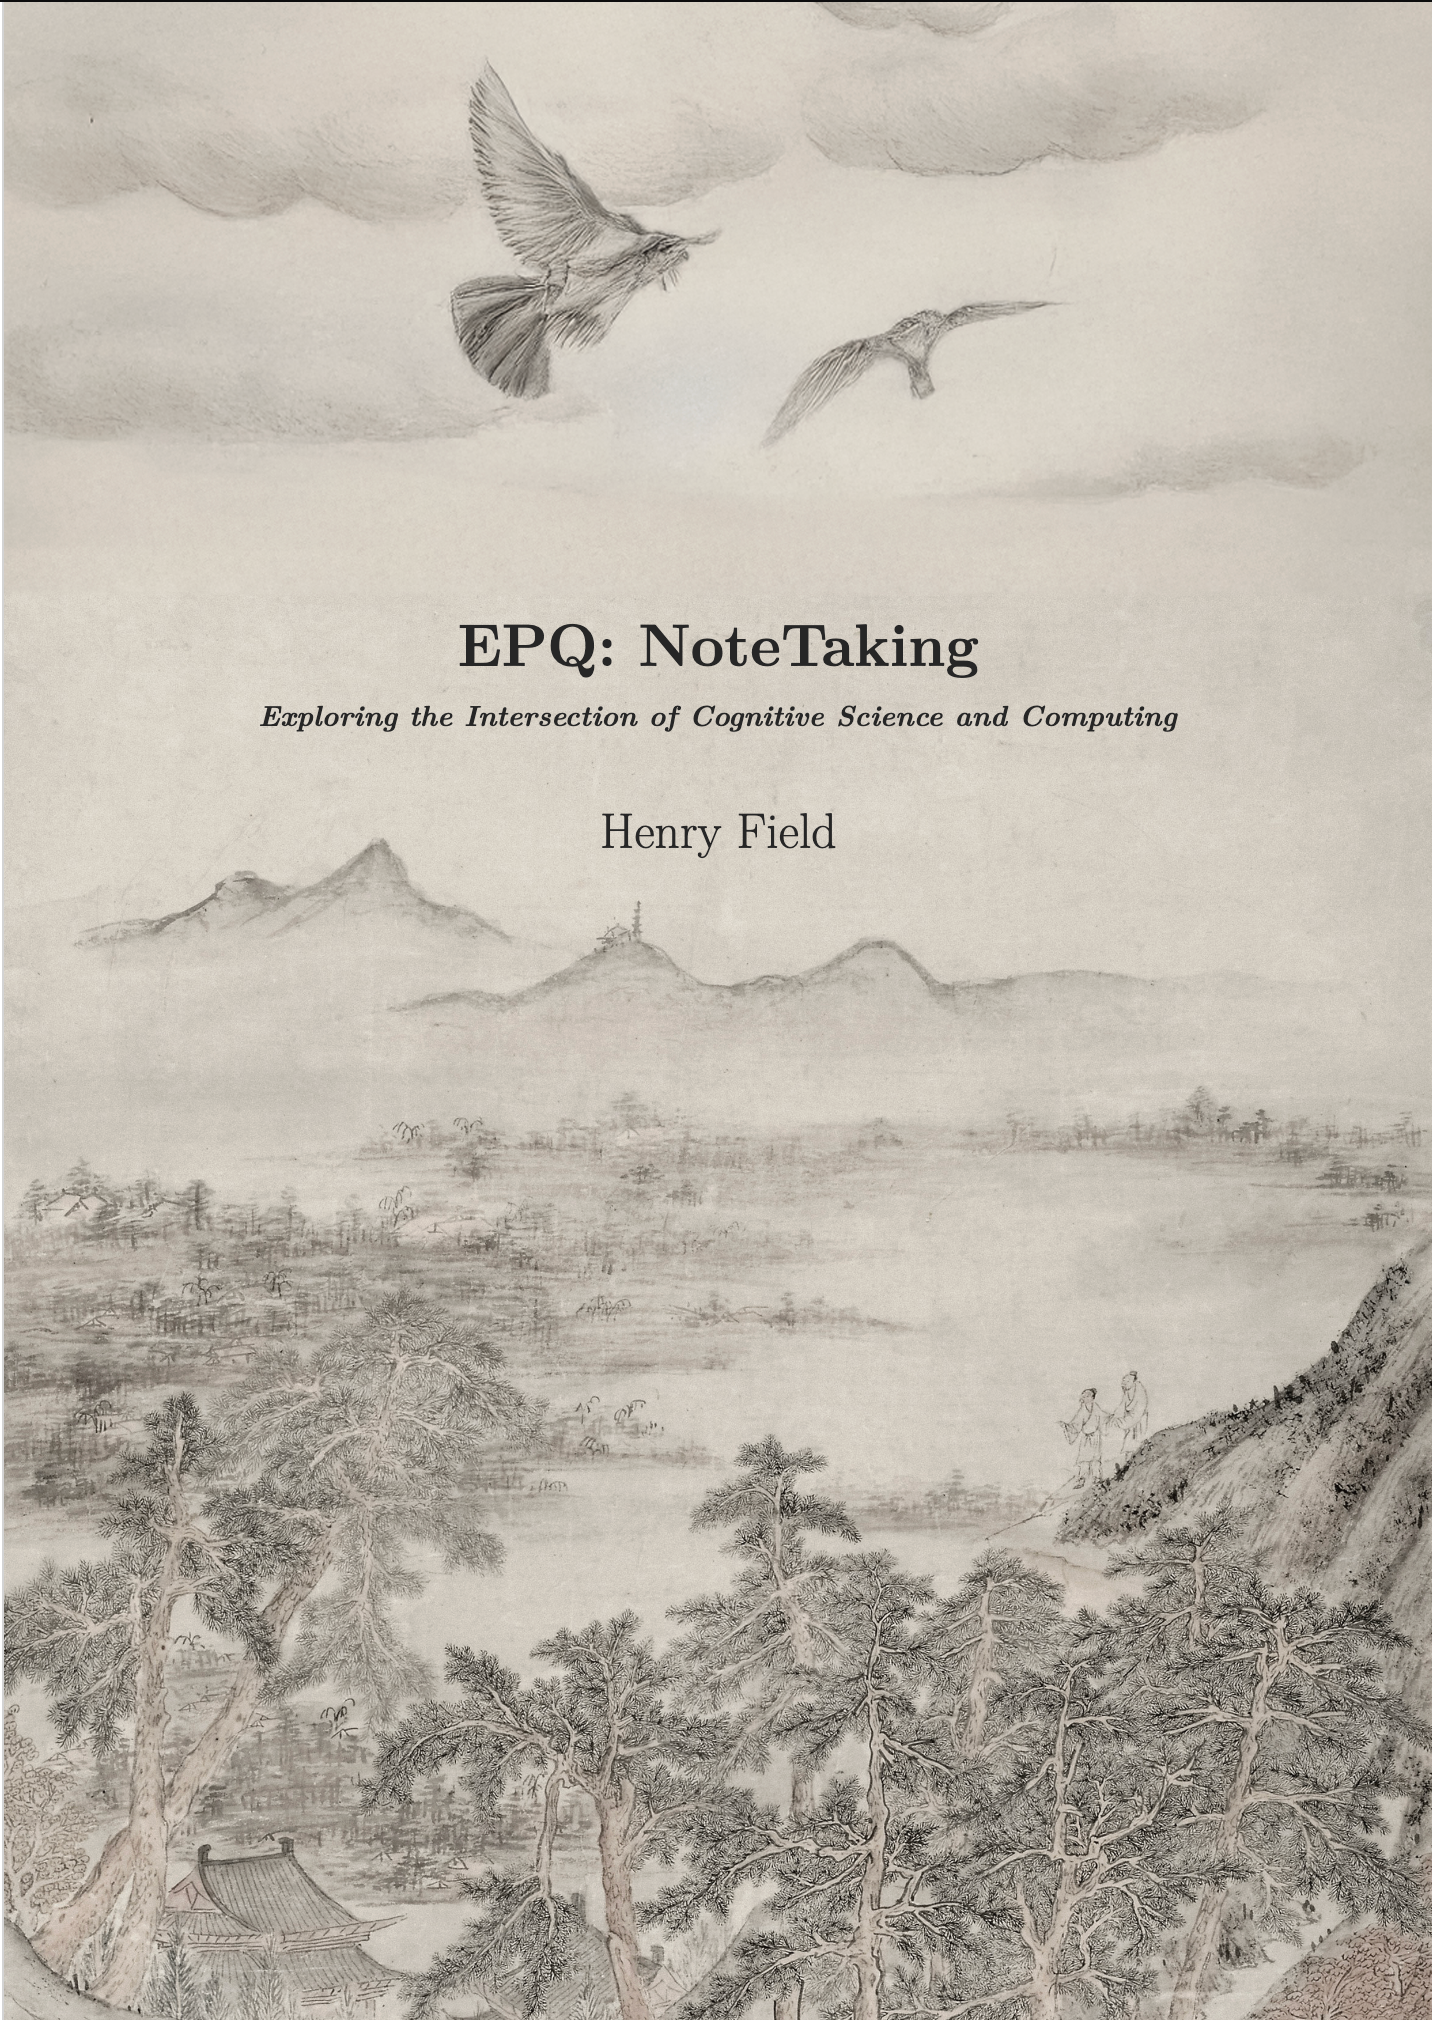
\includegraphics[width=0.6\textwidth]{Diary/35_WC_30-6-25/media/draftTitlePage.png}
    \caption{Draft title page for my report}
\end{figure}

I really like this image as it represents the Japanese belief of dependence on nature for man's success and happiness, which I feel is a great representation of my project which looks to built on this natural dependence to built on productivity and focus. Whilst it may seem counterintuitive to use a natural image for such a digital project I feel that it is a great representation of the balance between nature and technology that my project aims to achieve.

\subsection*{Plans for next week:}
Next week I will continue to migrate my report documentation to \LaTeX{}.